\chapter{辐射场的几何与物理描述}

辐射场的宏观描述是天体物理研究的基础,这一章会定义描述辐射场的基本物理量，并探讨一些基本规律。
\section{基本物理量}

为了定量描述辐射场，我们需要引入四个核心物理量：辐射强度、辐射流量、辐射能量密度和辐射压。

\subsection{辐射强度}

辐射强度是描述辐射场最基本的量，它包含了辐射在空间位置、方向、频率上的所有信息。
\n{补个图}
\begin{definition}[单色辐射强度]
    考虑辐射场中任意一点，取一面元 $dA$，其法线方向为 $\mathbf{n}$。设在时间间隔 $dt$ 内，频率范围在 $\nu$ 到 $\nu + d\nu$ 之间，穿过该面元并限制在方向 $\mathbf{n}'$ 周围立体角 $d\Omega$ 内的辐射能量为 $dE_\nu$。则单色辐射强度 $I_\nu$ 定义为：
    \begin{equation}
        I_\nu = \frac{dE_\nu}{dA \cos\theta \, dt \, d\Omega \, d\nu}
    \end{equation}
    其中 $\theta$ 是辐射传播方向 $\mathbf{n}'$ 与面元法线 $\mathbf{n}$ 之间的夹角，$dA \cos\theta$ 代表面元在垂直于传播方向上的投影面积。
\end{definition}
\n{单位：$\mathrm{erg s^{-1} cm^{-2}  sr^{-1} Hz^{-1}}$}
\begin{figure}
    \centering
    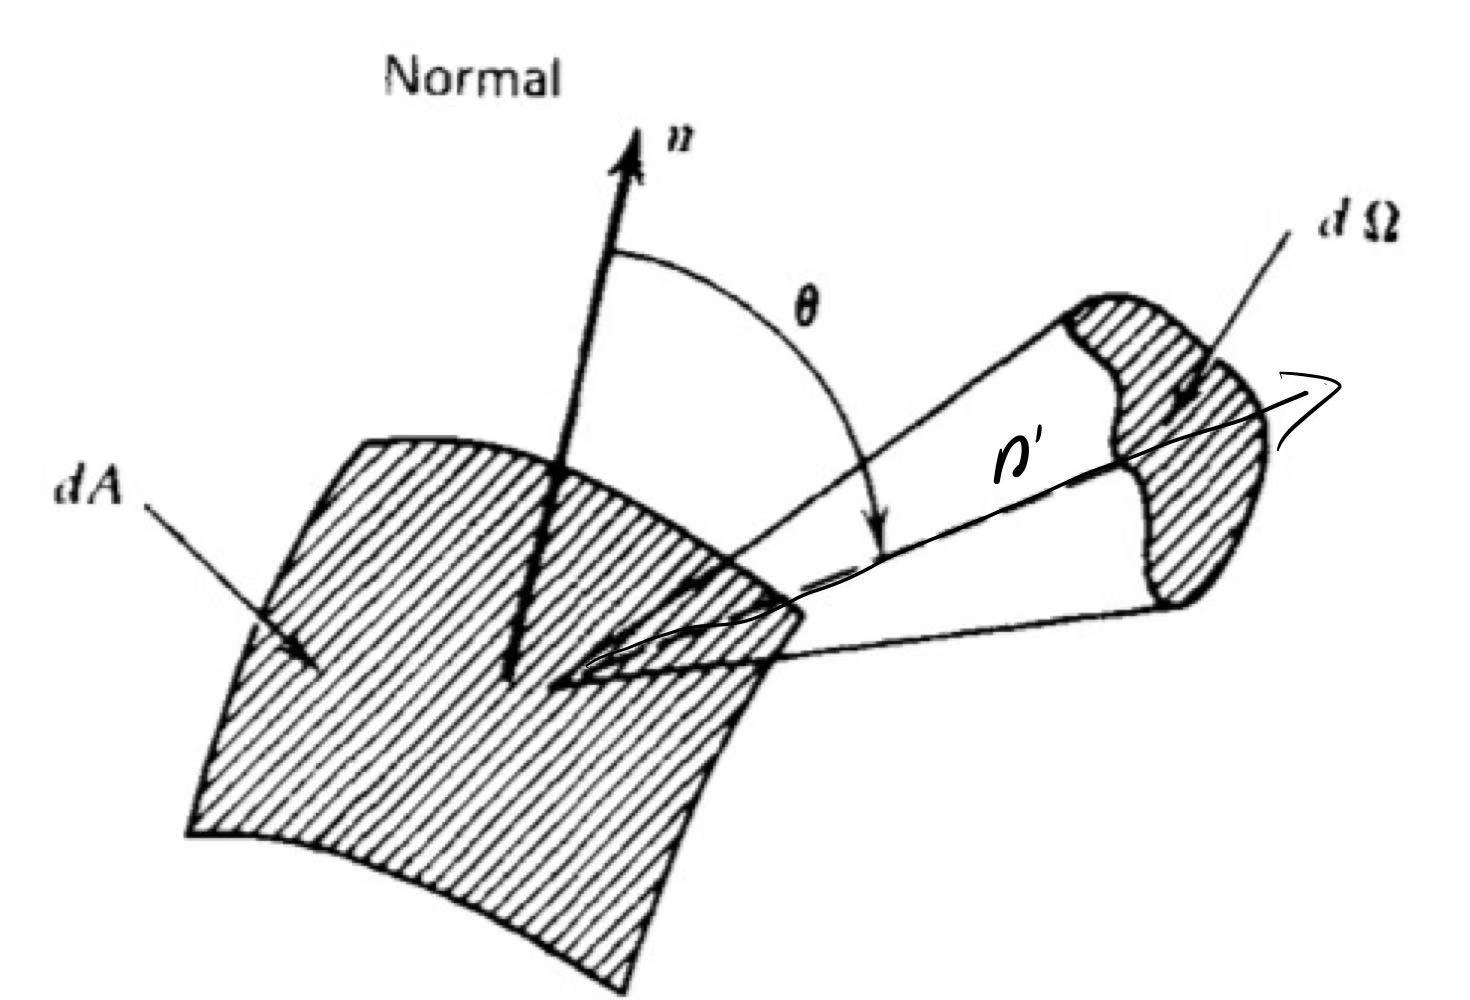
\includegraphics[width = .5\linewidth]{figs/Intensity.jpg}
    \caption{辐射强度示意图}
\end{figure}

辐射强度 $I_\nu(r, n, t)$ 一般是位置、方向和时间的函数。如果 $I_\nu$ 与方向无关，则称辐射场是各向同性的；如果 $I_\nu$ 不随位置变化，则称辐射场是均匀的；
如果 $I_\nu$ 不随时间变化，则称辐射场是稳定的。

单色辐射强度对频率积分便可得总辐射强度：
$$
    I = \int I_\nu d\nu
$$

\subsection{辐射流量}

辐射强度描述了特定方向的辐射能力，而辐射流量则关注通过某一表面的净能量流。

\begin{definition}[单色辐射流量]
    单色辐射流量 $F_\nu$ 定义为单位时间内、单位频率间隔内穿过单位面积的净能量：
    \n{但是计算黑体表面辐射的时候，$\theta$只取到$\pi/2$。}
    \begin{equation}
        F_\nu = \int_{\Omega} I_\nu \cos\theta \, d\Omega
    \end{equation}
    
    积分范围通常为整个球立体角（$4\pi$）。
\end{definition}
\n{单位：$\mathrm{erg \cdot s^{-1} \cdot cm^{-2} \cdot Hz^{-1}}$}
若选择以面元法线方向为z轴的球坐标：
\begin{equation}
    F_\nu = \int_{0}^{2\pi} d\varphi \int_0^{\pi} I_\nu(\theta, \varphi) \cos{\theta} \sin{\theta} d\theta
\end{equation}
若辐射场是各向同性的（$I_\nu$ 为常数），则通过任意平面的净流量 $F_\nu = 0$，因为穿入和穿出的能量相互抵消。若仅计算穿过平面一侧（半球空间）的流量，则有：
\begin{equation}
    F_\nu^+ = \int_{0}^{2\pi} d\varphi \int_{0}^{\pi/2} I_\nu \cos\theta \sin\theta \, d\theta = \pi I_\nu
\end{equation}

如果讲辐射流量对面元做积分，就得到辐射源单色频率的功率，也称为单色光度。
\begin{definition}[单色光度]
    单位时间内、频率$\nu$处单位频率间隔内的辐射能量：
    \begin{equation}
        L_\nu = \int F_\nu dA = \int dA \int I_\nu \cos{\theta} d\Omega
    \end{equation}
    单色光度对频率积分便得到总辐射功率，也称为光度：
    \begin{equation}
        L = \int d\nu L_\nu
    \end{equation}
\end{definition}
\begin{figure}[H]
    \centering
    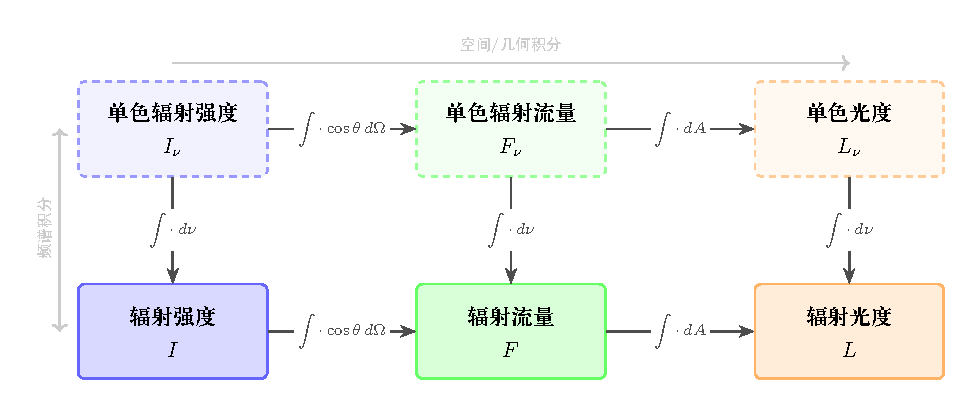
\includegraphics[width = \linewidth]{figs/fig_quantities.pdf}
    \caption{强度、流量和光度之间的关系}
\end{figure}
\subsection{辐射能量密度}

能量密度描述了单位体积内储存的辐射能量。
\n{单位：$\mathrm{erg \cdot cm^{-3} \cdot Hz^{-1}}$}
\begin{definition}[单色能量密度]
    单色能量密度 $u_\nu$ 定义为单位体积内、单位频率间隔内的辐射能量。
    \begin{equation}
        u_\nu = \frac{1}{c} \int_{4\pi} I_\nu \, d\Omega = \frac{4\pi J_\nu}{c}
    \end{equation}
    其中 $c$ 为光速，$J_\nu$是方向平均的辐射强度：
    \begin{equation}
        J_\nu = \frac{1}{4\pi} \int_\Omega I_\nu (\theta, \varphi) d\Omega
    \end{equation}
\end{definition}

\begin{definition}[总能量密度]
    总能量密度是单色能量密度对频率的积分：
    \begin{equation}
        u = \int_\nu u_\nu d\nu = \frac{4\pi}{c}\int J_\nu d\nu \\
    \end{equation}
\end{definition}

对于各向同性辐射场，积分简单地给出：
\begin{align}
    u_\nu &= \frac{4\pi}{c} I_\nu \\
    u &= \frac{4\pi}{c} I
\end{align}
这表明各向同性场的能量密度仅由辐射强度决定。

\begin{figure}[H]
    \centering
    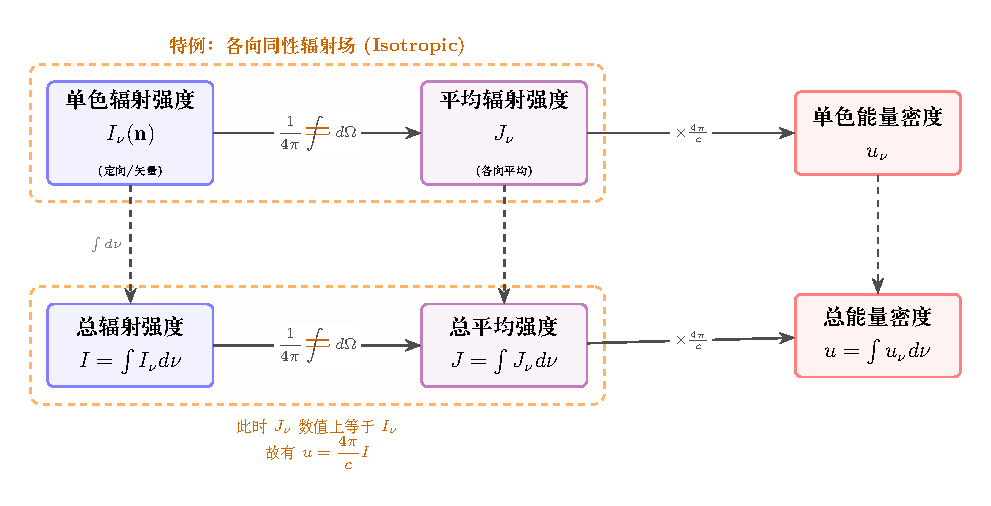
\includegraphics[width = \linewidth]{figs/fig_intensity_density.pdf}
    \caption{辐射强度、平均强度和能量密度}
\end{figure}
\n{此关系恒成立：$u = \frac{4\pi}{c}J$}
\begin{derivationnote}[为什么能量密度要除以 $c$？]
    考虑一束沿法线方向穿过面元 $dA$ 的辐射。根据辐射强度的定义，在微小时间间隔 $dt$ 内，穿过该面元的辐射能量为：
    \begin{equation*}
        dE = I_\nu \, dA \, dt \, d\Omega \, d\nu
    \end{equation*}
\n{或者可以理解为，流量=密度$\times$速度}
\begin{figure}[H]
    \centering
    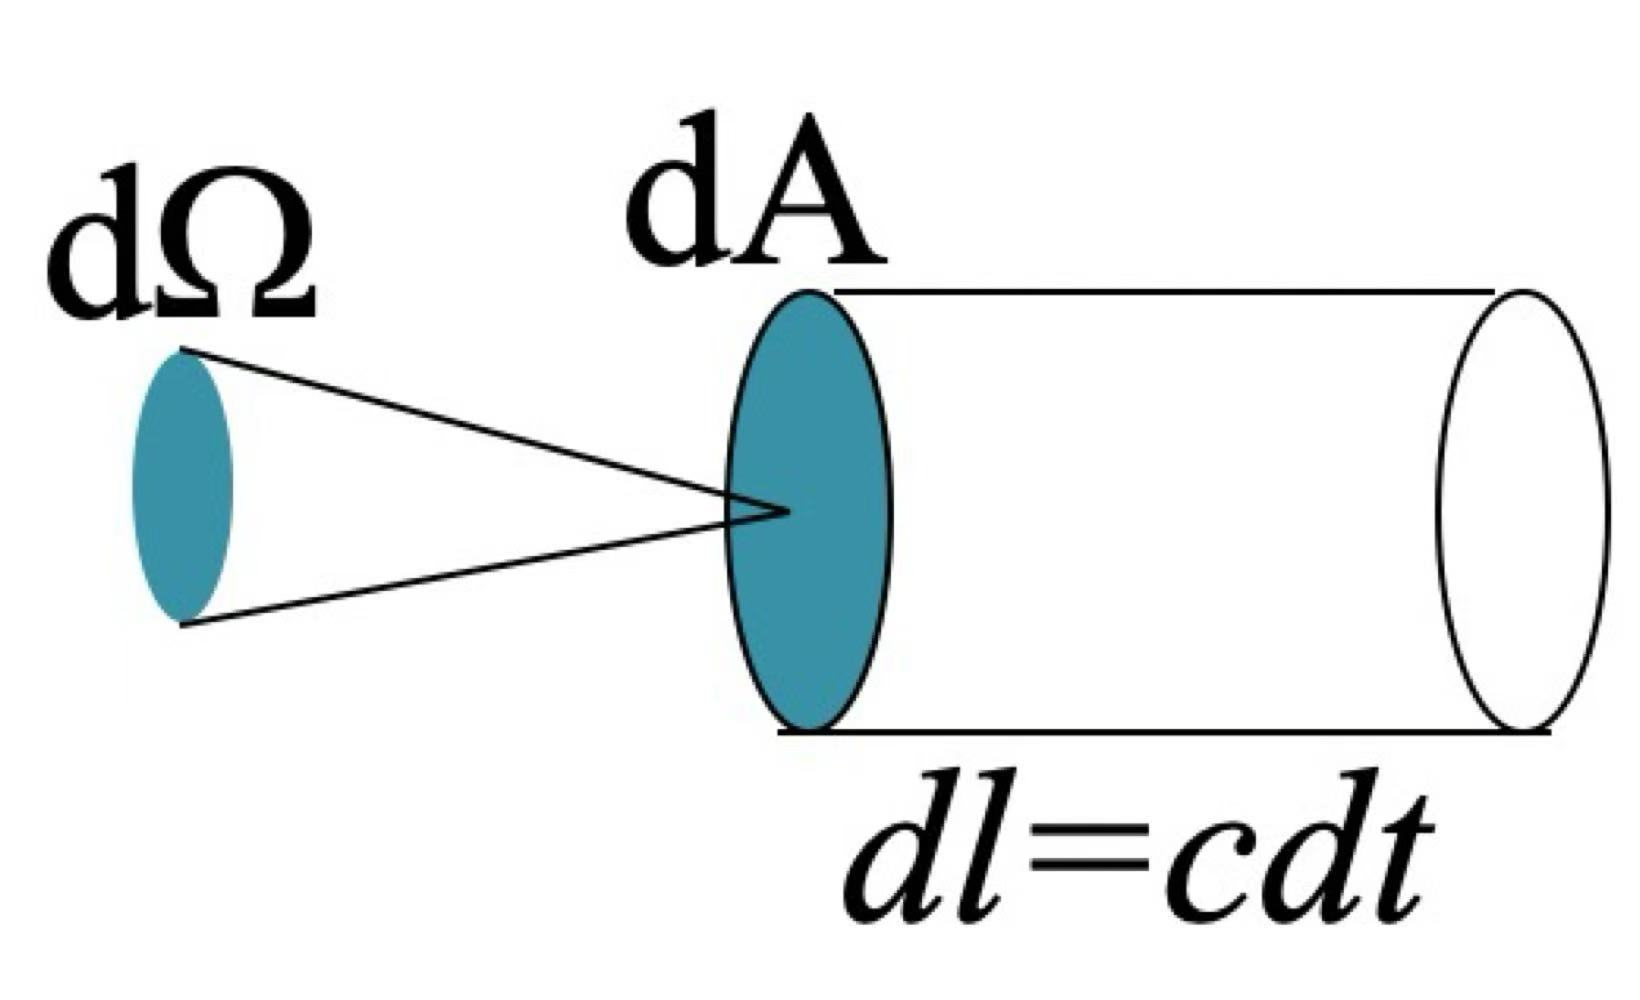
\includegraphics[width = .3\linewidth]{figs/fig_intensity_density.jpg}
    \caption{能量密度和辐射强度}
\end{figure}
    在这段时间 $dt$ 内，以光速 $c$ 传播的光子向前行进的距离为 $L = c \cdot dt$。这意味着，刚刚穿过面元 $dA$ 的这部分能量 $dE$，实际上填充了一个底面积为 $dA$、高为 $c \cdot dt$ 的柱体空间。该柱体的体积为：
    \begin{equation*}
        dV = dA \cdot (c \cdot dt)
    \end{equation*}
来自该方向的辐射对能量密度的贡献为：
    \begin{equation*}
        u_\nu(\Omega) = \frac{\text{能量}}{\text{体积}} = \frac{I_\nu \, dA \, dt \, d\Omega \, d\nu}{dA \cdot (c \cdot dt) \, d\Omega \, d\nu} = \frac{I_\nu}{c}
    \end{equation*}
\end{derivationnote}


\subsection{辐射压}

光子携带动量，因此辐射照射在物体表面会产生压强。光子的动量大小为 $p = E/c$，用牛顿方程可以计算出辐射压。
\n{这里假设光子把全部动量都传递到接受面，比如全部吸收。}
\begin{theorem}[单色辐射压公式]
    单色辐射压 $P_\nu$ 定义为辐射场中动量流密度在面元法线方向的分量。对于辐射强度为 $I_\nu$ 的辐射场，其计算公式为：
    \begin{equation}
        P_\nu = \frac{1}{c} \int_{4\pi} I_\nu \cos^2\theta \, d\Omega
    \end{equation}
\end{theorem}

\begin{proof}
    根据辐射强度的定义，在时间间隔 $dt$ 内，从方向 $(\theta, \phi)$ 的立体角 $d\Omega$ 穿过法向面元 $dA$ 的辐射能量为：
    \n{第一个 $\cos\theta$，源于面元在辐射传播方向上的\textbf{投影面积}。}
    \begin{equation*}
        dE_\nu = I_\nu \cos\theta \, dA \, dt \, d\Omega
    \end{equation*}
    能量为 $dE$ 的光子携带的动量大小为 $dp = dE/c$，动量沿着面元法线方向的分量 $dp_{\perp}$：
    \n{第二个 $\cos\theta$，源于\textbf{投影动量}。}
    \begin{equation*}
        dp_{\perp} = dp \cdot \cos\theta = \frac{dE}{c} \cos\theta
    \end{equation*}
    
    
    代入 $dE_\nu$：
    \begin{equation*}
        dp_{\perp} = \frac{1}{c} (I_\nu \cos\theta \, dA \, dt \, d\Omega) \cdot \cos\theta = \frac{1}{c} I_\nu \cos^2\theta \, dA \, dt \, d\Omega
    \end{equation*}
    
    根据压强定义 $P_\nu = \frac{dp_{\perp}}{dA \, dt}$ ,对全立体角积分即得：
    \begin{equation*}
        P_\nu = \int_{4\pi} \frac{1}{c} I_\nu \cos^2\theta \, d\Omega
    \end{equation*}
\end{proof}
如果考虑反射面的辐射压，法向动量在出射时变化量是两倍的入射法向量，此时辐射压为：
\begin{equation}
    P_\nu = \frac{2}{c}\int_0^{2\pi}d\varphi \int_o^{\pi/2}I_\nu(\theta, \varphi) \cos{\theta}^2\sin{\theta}d\theta
\end{equation}
如果考虑各向同性的情况，不难计算得：
\begin{align}
    p_\nu &= \frac{4\pi I_\nu}{3c} \\
    P &= \int p_\nu d\nu = \frac{4\pi I}{3c}
\end{align}

\n{这点不难从之前的计算中看出来}
\begin{theorem}[辐射压和辐射密度的关系]
    对于各向同性的辐射场，辐射压与能量密度之间存在确定的关系：
    \begin{equation}
        P_\nu = \frac{1}{3} u_\nu
    \end{equation}
\end{theorem}


\section{辐射在自由空间中的传播}

在没有吸收、发射或散射的真空中，辐射场的演化遵循简单的几何守恒律。

\begin{theorem}[强度不变原理]
    在真空（或折射率为常数的介质）中，沿光线传播方向，单色辐射强度保持不变。即对于光线上的任意两点 $r_1$ 和 $r_2$，有：
    \begin{equation}
        I_\nu(r_1) = I_\nu(r_2)
    \end{equation}
\end{theorem}

\begin{proof}
    考虑一束光线穿过两个面元 $dA_1$ 和 $dA_2$，两者距离为 $R$，且均垂直于光线传播方向。
    
    面元 $dA_1$ 对 $dA_2$ 张开的立体角为 $d\Omega_1 = dA_2 / R^2$。
    
    面元 $dA_2$ 对 $dA_1$ 张开的立体角为 $d\Omega_2 = dA_1 / R^2$。
    
    根据能量守恒，在没有能量损失的真空中，流出 $dA_1$ 并射向 $dA_2$ 的能量 $dE_1$ 必须等于 $dA_2$ 接收到的能量 $dE_2$。
    \begin{align}
        dE_1 &= I_\nu(r_1) dA_1 dt d\Omega_1 d\nu \\
        dE_2 &= I_\nu(r_2) dA_2 dt d\Omega_2 d\nu
    \end{align}
    令 $dE_1 = dE_2$，并代入立体角的几何关系：
    \begin{equation}
        I_\nu(r_1) dA_1 \left( \frac{dA_2}{R^2} \right) = I_\nu(r_2) dA_2 \left( \frac{dA_1}{R^2} \right)
    \end{equation}
    消去两边的几何因子 $dA_1 dA_2 / R^2$，即得 $I_\nu(r_1) = I_\nu(r_2)$。
\end{proof}

\begin{theorem}[平方反比律]
    对于一个光度为 $L$ 的各向同性点源（或球对称源），距离源 $r$ 处的辐射流量 $F$ 与距离的平方成反比：
    \begin{equation}
        F = \frac{L}{4\pi r^2}
    \end{equation}
\end{theorem}

\begin{proof}
    考虑以源为中心、半径为 $r$ 的球面。根据能量守恒，单位时间内穿过该球面的总能量必须等于源的辐射总功率（光度）$L$。
    
    由于源是各向同性的，球面上各点的流量 $F$ 相等，且方向沿径向向外（$\cos\theta = 1$）。总光度为流量对球面积分：
    \begin{equation}
        L = \int_{\text{sphere}} F \, dA = F \cdot (4\pi r^2)
    \end{equation}
    移项即得 $F = L / (4\pi r^2)$。
\end{proof}
对于一个半径为 $R$、表面均匀亮度为 $I$ 的球形天体，在距离 $r$ ($r \gg R$) 处的观测者测得的流量为：
\begin{equation}
    F = \int_{\text{source}} I \cos\theta \, d\Omega \approx I \cdot \Omega_{\text{source}} = I \cdot \frac{\pi R^2}{r^2}
\end{equation}
\n{各向同性，只考虑表面辐射通量为 $F = \pi I$}
这与平方反比律 $F = (4\pi R^2 \cdot \pi I) / (4\pi r^2)$ 的结果是一致的。